\section{Applications}
\label{sec:Apps}
Many applications in scientific computing typically employ double precision when lower precision may actually be sufficient. 
Due to the advances in processors, FLOPs are now considered free, causing bandwidth and storage to be the computational bottleneck. 
With the emergence of new technology that supports low precision and the need to reduce bandwidth and storage concerns, interest in mixed-precision algorithms has reemerged. 
%However, identifying which applications can tolerate lower precision and still achieve sufficient results is a challenging task that wasn't particularly relevant prior to the emergence of new technology that supports low precision.

Since low and mixed precision settings benefit from speed-up and reduced storage, applications that process large amounts of data are potential candidates for this research.
Here, we discuss our results from applying our mixed-precision HQR as a subroutine of an iterative eigensolver in the context of spectral clustering.\par

\paragraph{Graph partitioning} A graph is defined by a set of nodes and a set of edges between the nodes.
Partitioning, or clustering, is a task that seeks communities within a graph such that nodes within a community are \emph{more similar} to each other than to nodes outside of that community. 
In datasets where the true communities are known, we can use pairwise-precision and pairwise-recall (see \cite{GraphChallenge})  which are defined in Definition~\ref{def:P&R}) to evaluate the accuracy of a clustering task.
\begin{definition}
	\label{def:P&R}
	%Some relevant evaluation metrics of classification of clustering tasks are precision and recall. 
	%Precision is the fraction of relevant instances among the retrieved instances.
    Pairwise-precision and pairwise-recall are measured by checking for every pair of nodes if the pair is classified into the same cluster (positive), or else (negative).
	\begin{equation}
	\text{Precision} = \frac{\#\text{True Positive}}{\#\text{True Positive}+\#\text{False Positive}}, 
	\qquad
	%%% \end{equation} 
	%Recall is the fraction of relevant instances that have been retrieved over the total amount of relevant instances.
	%%% \begin{equation}
	\text{Recall} = \frac{\#\text{True Positive}}{\#\text{True Positive}+\#\text{False Negative}}.
	\end{equation}
\end{definition}

\subsection{Spectral Graph Clustering}
\label{sec:cluster}
Some spectral clustering methods utilize identifying $k$ dominant eigenvectors of a similarity matrix of a graph, which then can be used to identify $k$ clusters. 
Another potential use of iterative eigensolvers for spectral clustering is in identifying the second smallest eigenvalue and its eigenvector pair, called the Fiedler value and vector.
%Whether convergence to the Fiedler vector is quick or not is more uncertain than in identifying dominant eigenvectors.
In addition, many eigenproblems outside of spectral clustering only require finding a few eigen pairs.
This family of problems tends to admit tall-and-skinny matrix structures and could utilize TSQR as well. 
We will use subspace iteration, a variant of the power method defined in Algorithm~\ref{algo:subIter} that uses a QR factorization of a tall-and-skinny matrix at each iteration and that quickly converges to the dominant eigenvectors.
Although we only experimented with comparing mixed-precision HQR to uniform precision HQR, TSQR could also be used in this application. 
\par

\subsubsection{Subspace Iteration}
Subspace iteration is a modification of the power method, which computes an invariant subspace with dimension $p > 1$ (see \cite{Bai2000}).
A variant of this algorithm is shown below in Algorithm~\ref{algo:subIter}.

\begin{algorithm2e}
	\DontPrintSemicolon % Some LaTeX compilers require you to use \dontprintsemicolon instead
	\KwIn{Adjacency matrix $\bb{A}\in\{0, 1\}^{m \times m}$ where $m \geq n$, {\tt max\_iter}, the maximum number of iterations, $\tau$ the threshold for the eigenspace error, and $k$, the suspected number of clusters.}
	\KwOut{$\bb{Q}$}
	Initialize $\bb{Y}\in \mathbb{R}^{m\times k}$, a random matrix.
	\tcp{$Y$ would likely be full-rank.} 
	$\bb{Q}, \bb{R}\gets \tt{qr}(\bb{Y})$ 
	\For{$i=1, \cdots,$ {\tt max\_iter}}{
		$\bb{Y} \gets \bb{AQ}$\;
		\If{$\frac{\|\bb{Y}-\bb{QQ}^{\top}\bb{Y}\|_2}{\|\bb{Y}\|_2} < \tau$}{exit loop. \tcp{$\|\bb{Y}-\bb{QQ}^{\top}\bb{Y}\|_2$ is the eigenspace error.}}
		$\bb{Q, R} \gets {\tt qr}(\bb{Y})$
	}
	\Return $\bb{Q}$
	\caption{$\bb{Q}=$ {\tt subIter}$(\bb{A}, \text{\tt max\_iter}, \tau, k)$. Find orthogonal basis (given by columns of output matrix $Q$) of an invariant subspace of the input adjacency matrix, $A$.}
	\label{algo:subIter}
\end{algorithm2e}
This algorithm is an iterative method with two possible stopping criteria: 1) the maximum number of iterations to complete before exiting the loop is declared as max\_iter, or 2) if the eigenspace error is smaller than $\tau$, then exit the loop.
In practice, we added a third stopping criterion in the case that the declared $\tau$ value was too small, which would force an exit from the loop when the eigenspace error began to increase.

\subsubsection{Density-based Spatial clustering of Applications with Noise (DBSCAN)}
DBSCAN is a density-based spatial clustering algorithm introduced in \cite{EKSX1996} and is widely used in practice.
This algorithm only requires input data, location of nodes, and two parameters, radius of neighborhoods and minimum number of points required to form a dense region. 
The two parameters for the DBSCAN algorithm were tuned to provide the best result, given that we used the same set of parameters for the entire experiment.

\subsection{Experiment Details and Results}
Our main goal in this experiment was to test if the eigenspaces identified by lower precision HQR could produce sufficient graph partitioning. 
We used subspace iteration (Algorithm~\ref{algo:subIter}) to identify eigenspaces, DBSCAN to partition the embedding of the nodes onto these eigenspaces, and precision and recall to evaluate clustering performances. 
We used a static graph of $5000$ nodes  with $19$ known true partitions for the Graph Challenge \cite{GraphChallenge}, which are derived from block stochastic matrices. 
The graphs we used were undirected and unweighted; the only elements in the adjacency matrices were $0$'s and $1$'s, which can easily be represented in half, single, and double precision floats. 
For $i=1, \cdots, 10$, let $\bb{Y}_{\text{half},i}\in\F_{\text{half}}^{5000\times 19}$ be the half precision storage of the $i^{th}$ random matrix.
Since any half precision float can be exactly represented in single and double precisions, $\bb{Y}_{\text{half},i}$'s can be easily cast up to single and double precisions, $\bb{Y}_{\text{single},i}$ and $\bb{Y}_{\text{double},i}$.
We performed mixed-precision HQR within subspace iteration initialized by $\bb{Y}_{\text{half},i}$'s, and uniform-precision HQR for subspace iteration initialized by $\bb{Y}_{\text{single},i}$'s  and $\bb{Y}_{\text{double},i}$'s.
For trial $i = 1, \cdots, 10, $ we repeated the following steps.
\begin{enumerate}[Step 1.]
	\item Identify an orthogonal basis of dimension 19 (number of known true partitions) with subspace iteration using the appropriate HQR routine for $\bb{Y}_{\text{half},i}$, $\bb{Y}_{\text{single},i}$ and $\bb{Y}_{\text{double},i}$.
	\item Apply DBSCAN to the output matrices of previous step to cluster most nodes into communities and the remaining nodes as outliers. 
	\item Measure clustering performances of DBSCAN on the three different precision subspace iteration embeddings using precision and recall.
\end{enumerate}

\paragraph{Subspace Iteration Results} 
\begin{wrapfigure}{r}{.5\textwidth}
	\centering
	%\vspace{-10pt}
	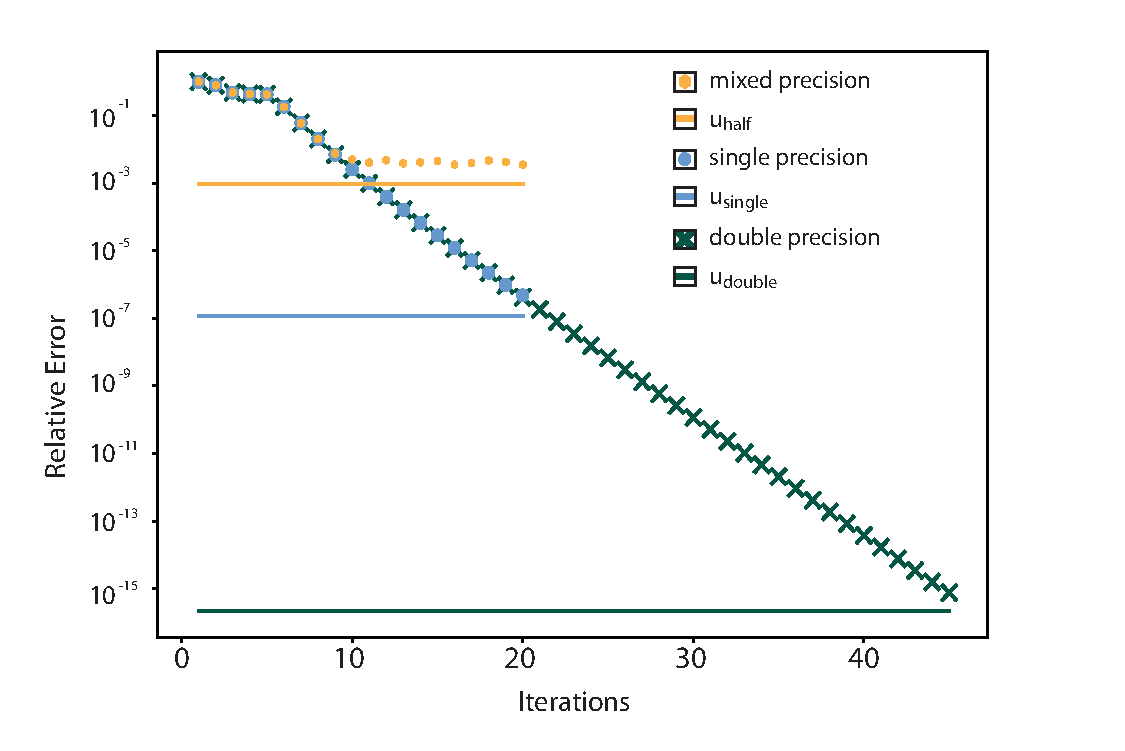
\includegraphics[width=.5\textwidth]{./figures/5000-19subIter.pdf}
	\caption{\label{fig:subIter} Eigenspace Error for subspace iteration with using double-, single-, and half- precision traditional Householder QR factorizations.}
	\vspace{-20pt}	
\end{wrapfigure}
Figure~\ref{fig:subIter} shows the eigenspace error, $\|\bb{Y}-\bb{QQ}^{\top}\bb{Y}\|_2/\|\bb{Y}\|_2$, from the subspace iteration step of one trial.
The stopping criteria, $\tau$, were set to $5u_{\text{single}}$ and $5u_{\text{double}}$ for the uniform precision HQRs and $5u_{\text{half}}$ for the mixed-precision HQR.
The solid lines are plotted to show the unit round-off values. 
The uniform precision implementations of subspace iterations reached their stopping criterion set by $\tau$, and the mixed-precision implementation fluctuated close to but never dipped below $\tau$. 
The convergence rate was approximately the same across the three different implementations, which suggests that the lower precision routines (mixed-precision HQR or uniform single precision HQR) can be used as a preconditioner for the double precision solution, and if paired with appropriate hardware could lead to increased computational efficiency.
In addition, if double precision eigenspace error is not necessary to achieve sufficient clustering results, we can simply use the lower precision HQR subspace iterations as full eigensolvers. 

\paragraph{Clustering Results} 
Table~\ref{table:PR} shows the worst-case precision and recall results from the $10$ trials for each subspace iteration implementation. 
The DBSCAN algorithm and the calculation of precision and recall were computed in double precision, and the variance in precision and recall values for these $10$ trials were in the range of {\tt 1e-6}.
Subspace iteration that employs lower precision HQR results in a suboptimal solution to the basis, which has a larger loss in orthogonality when compared to the solution from subspace iteration that uses higher precision HQR. 
However, clustering results show minimal difference in the precision and recall and suggests that a lower precision HQR within subspace iteration can still lead to a sufficiently accurate clustering. 
%Possible future works include trying different clustering methods for Step 2. 
\begin{table}[h!]
	\centering
%%% 	\begin{tabular}{ |c|c|c| } 
%%% 		\hline
%%% 		HQR scheme & Precision & Recall \\ \hline 
%%% 		mixed-precision & {\tt 0.9822} & {\tt 0.9393} \\ 
%%% 		single-precision & {\tt 0.9817} & {\tt 0.9407} \\ 
%%% 		double-precision &{\tt 0.9822} & {\tt 0.9405}\\
%%% 		\hline
%%% 	\end{tabular}
\begin{tabular}{ |c|c|c|c| }
\hline
HQR Scheme & Mixed Precision & Single Precision & Double Precision \\ \hline
Prec / Recall & 
{\tt 0.9822} / {\tt 0.9393} &
{\tt 0.9817} / {\tt 0.9407} &
{\tt 0.9822} / {\tt 0.9405} \\
\hline
\end{tabular}
	%%% \caption{\label{table:PR} Minimum (worst-case) precision and recall values for $10$ trials of DBSCAN on graph with $5000$ nodes and $19$ true clusters.}
	\caption{\label{table:PR} Minimum (worst-case) precision and recall for $10$ trials on graph with $5000$ nodes and $19$ true clusters.}
\end{table}
% and calls for further investigations into a variable precision approach to other spectral clustering methods as well.
%The mixed-precision implementation approached its best performance close to $10$ iterations, and continued to fluctuate near there without hitting the $\tau$ value. 
%Nonetheless, we can see that the first $9$ iterations of the subspace iteration technique yielded the same eigenspace errors for all three precisions. 
%The same pattern continued for single- and double- precision implementations until they reached single-precision unit round-off near $10^{-7}$, and the double-precision unit round-off near $10^{-15}$. 
%Therefore, we can do with lower-precision QR factorizations that require less storage and faster computation time if low-precision eigenspace error is sufficient for spectral clustering.
%Due to the random element of the initial matrix $\bb{Y}$ at the beginning of subspace iteration, there is some variability to its performance in identifying an invariant subspace. 
%In addition, we chose the number of columns of $\bb{Y}$ to be the number of true clusters, which is usually unknown in practice.
%\subsubsection{Results}
%We used the $5000$ node static graph from \cite{GraphChallenge}, but varied the clustering results by using $10$ different random matrices as the initial $\bb{Y}$.
%Therefore, for each HQR scheme (uniform double, uniform single, and mixed-precision) $10$ different initializations